
\section{Results}

In order to get a representation of the mechanism we run 300 randomly initiated scenarios. The experiemental setup is one such that it is possible to add more datapoints at a later date. From each simulation the no diagonal elements of the jacobian are used to construct a graph representative of the aggregated hourly means of the simulation output. Each of these graphs is then run through the infomap algorithm and a grouping/clustering produced. To select the best possible grouping, each infomap is run 100 times, where the result with the best fit (shortest codelength) is taken - this is an optional parameter on the algorithm.

\subsection{The co-grouping network}

To aggregate the groupings produced by each algorithm an $n\times n$ matrix is created for each of the $n$ species in the mechanism. This is treated as a graph relational matrix, whereupon if species A is in the same group as species B, then a link (or value +1) is added to the [A,B] (A\ce{->}B) and [B,A] (B\ce{->}A) column. Using this matrix format it is possible to then generate a graph showing the relationship between species that were clustered in the same group.

This relational matrix can then easily be converted into the network format: \autoref{fig:infomapprune}a. Starting with this it is then possible to filter edges below a certain weight, \autoref{fig:infomapprune}b-d. Finally isolates (nodes with no links) are removed, leaving only those clusters where each species has a strong relationship between every other. 

In the context of this section we select only relationships that appear in over 45\% of all the clustered simulation runs. The reasoning behind this is that there may exist a set of pairing that only appear either during the day or night.  

\begin{figure}[H]
\begin{subfigure}[t]{.5\textwidth}
  \centering
  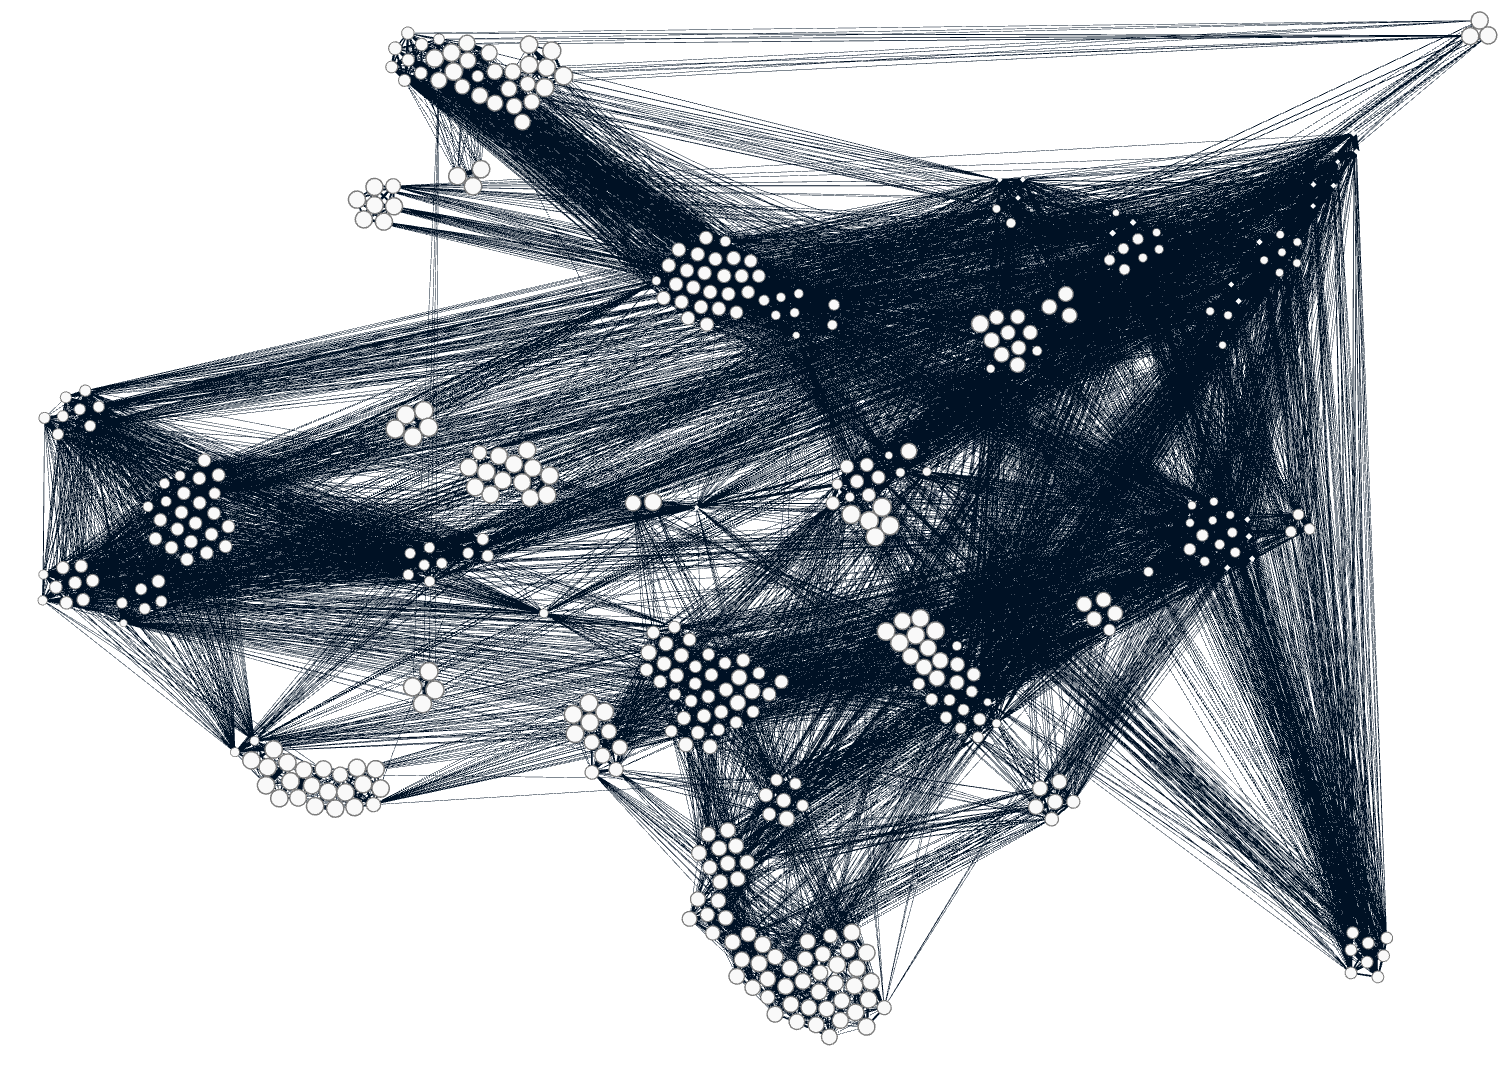
\includegraphics[width=\textwidth]{fig/c1.png}
  \caption{Full Graph}
\end{subfigure}%
\begin{subfigure}[t]{.5\textwidth}
  \centering
  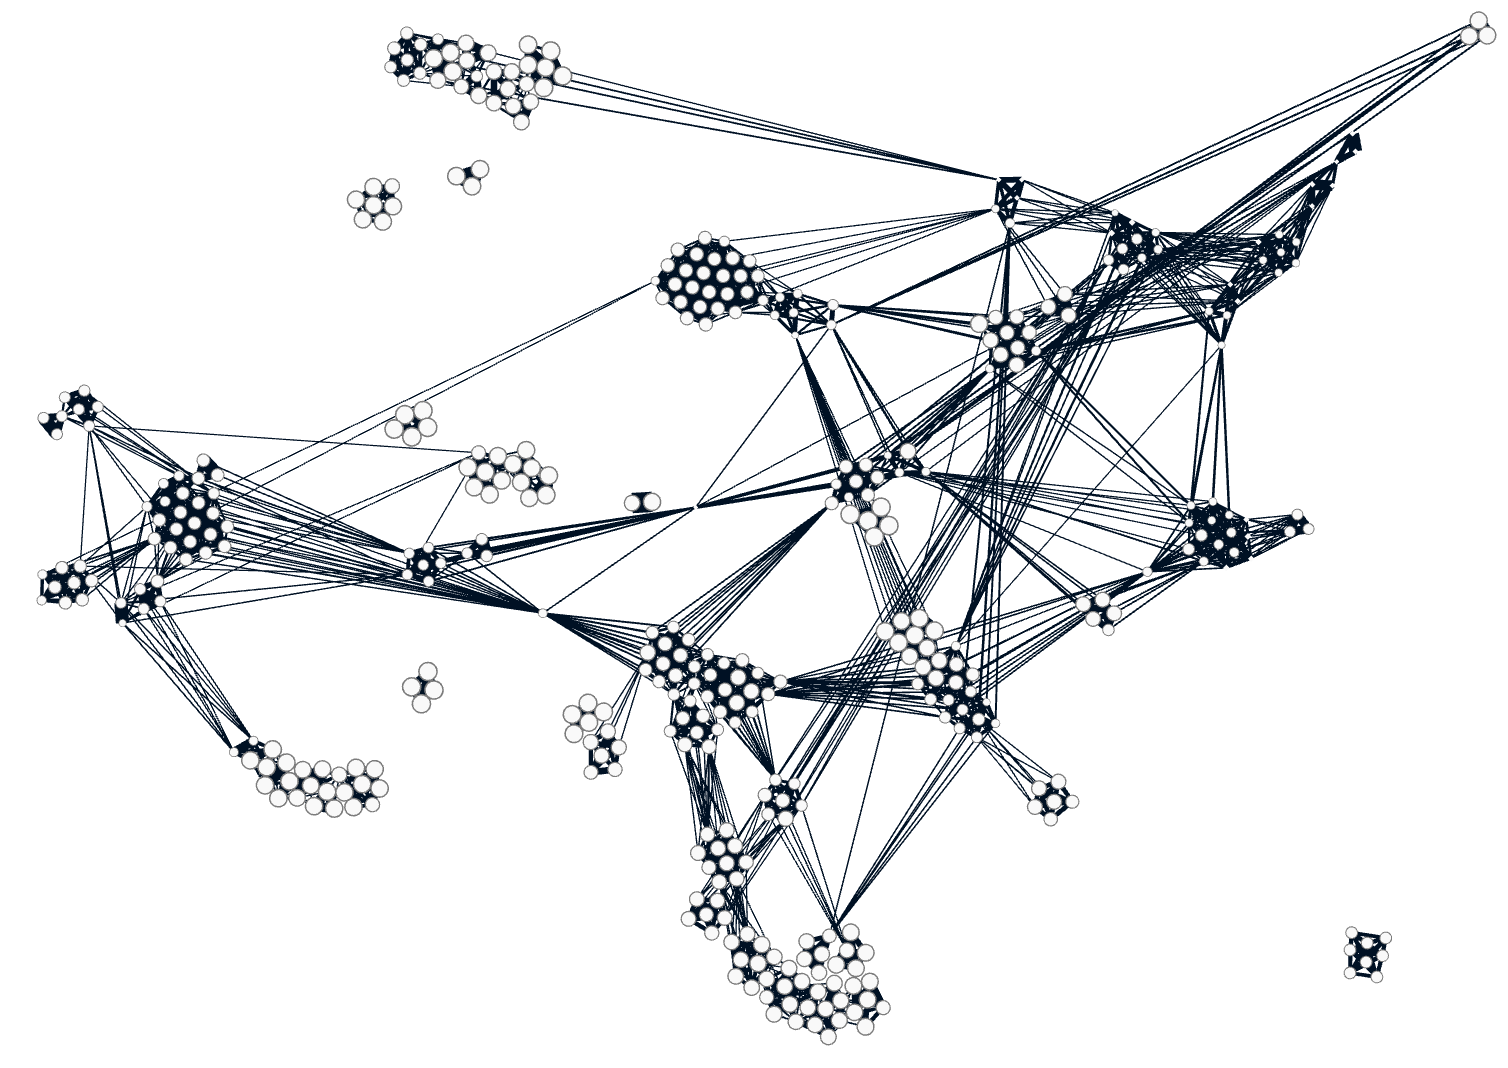
\includegraphics[width=\textwidth]{fig/c2.png}
  \caption{>10\% of graphs}
\end{subfigure}%\\

\begin{subfigure}[t]{.5\textwidth}
  \centering
  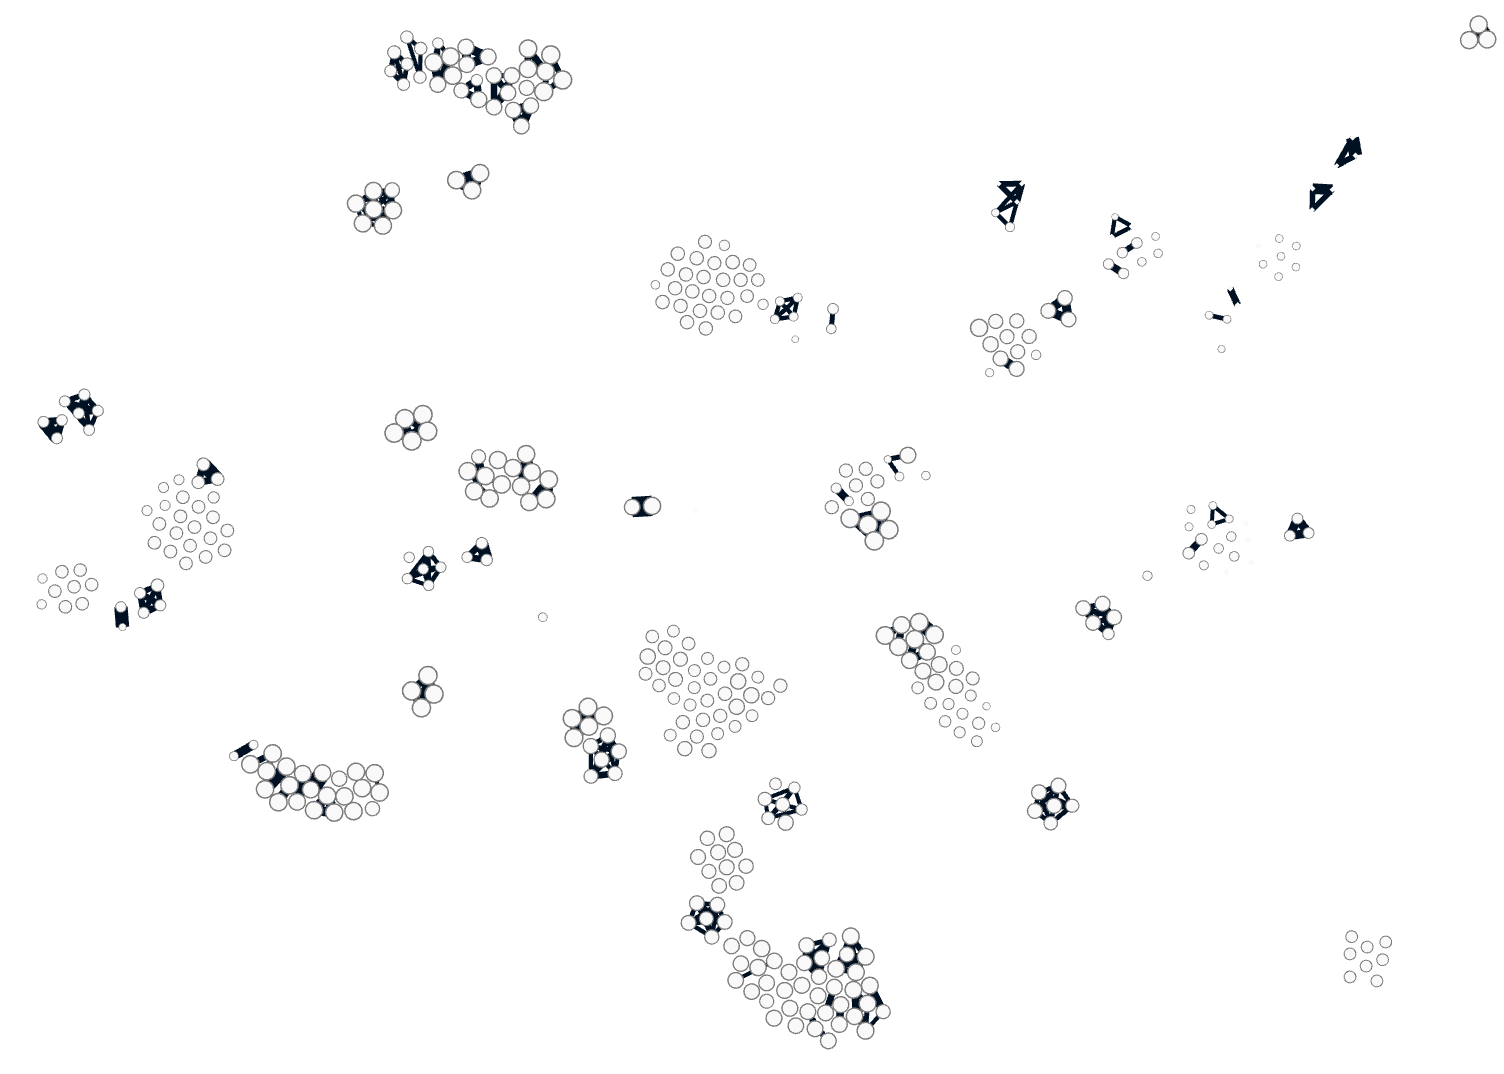
\includegraphics[width=\textwidth]{fig/c3.png}
  \caption{>20\%of graphs}
\end{subfigure}%
\begin{subfigure}[t]{.5\textwidth}
  \centering
  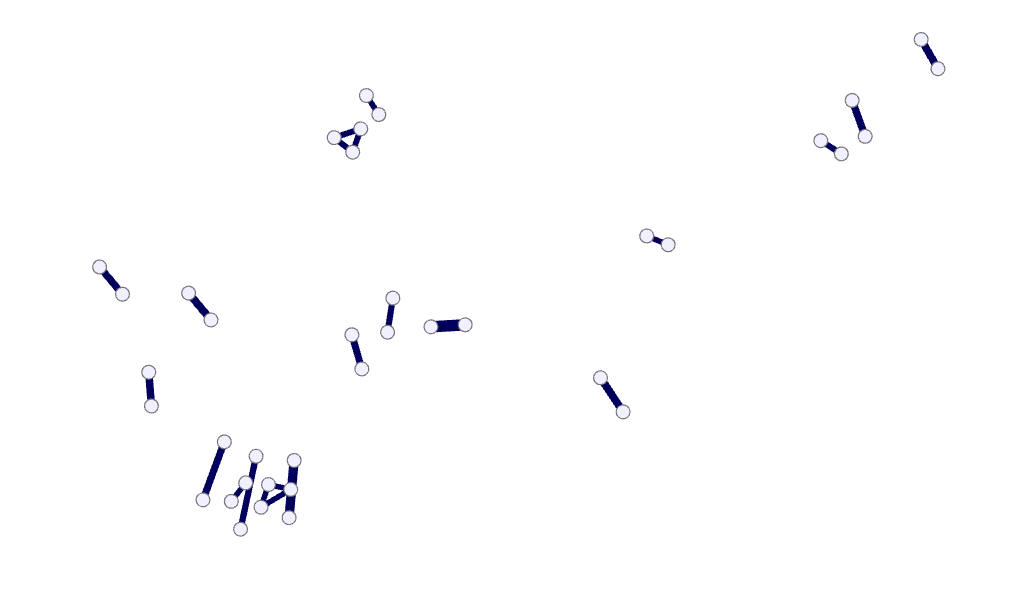
\includegraphics[width=\textwidth]{fig/c4.png}
  \caption{>40\%of graphs}
\end{subfigure}%
\caption{\textbf{Filetering the infomap clustering relationship matrix/graph} How the clutering relationship network changes as weak links (links between species which do not appear in many of the infomap groupings) are removed. }
\label{fig:infomapprune}
\end{figure}

\subsection{Comparing daytime and nightime groups}
In determing a group of species which are commonly custered together in most simulation results, we are next interested in seeing if these groups change with day or night. 

To do this we use an alluvial diagram. This is a cross between a parallel-line plot and a sanky diagram, and is particularly suitable for showing the changes in clusters within a temporal network, \citep{alluvial}.

In taking a the common clusters formed at midnight (\autoref{fig:alluvial} left)  and midday (\autoref{fig:alluvial} right) we are able to compare these to the overall selection (all hours - middle). Here, as is expected, any parings which persist in over 45\% of all the timesteps, exist in all three categories. In addition we see a selection of species which are grouped together at both 12:00 and 0:00 hours. This suggests that they may not be grouped with some of the intermediate hours, and that if the threshold of selection is lowered below 45, they may appear in the overall result. Finally a selection of species which are only grouped togehter in daytime or night time only results.



\begin{figure}%[H]
    \centering
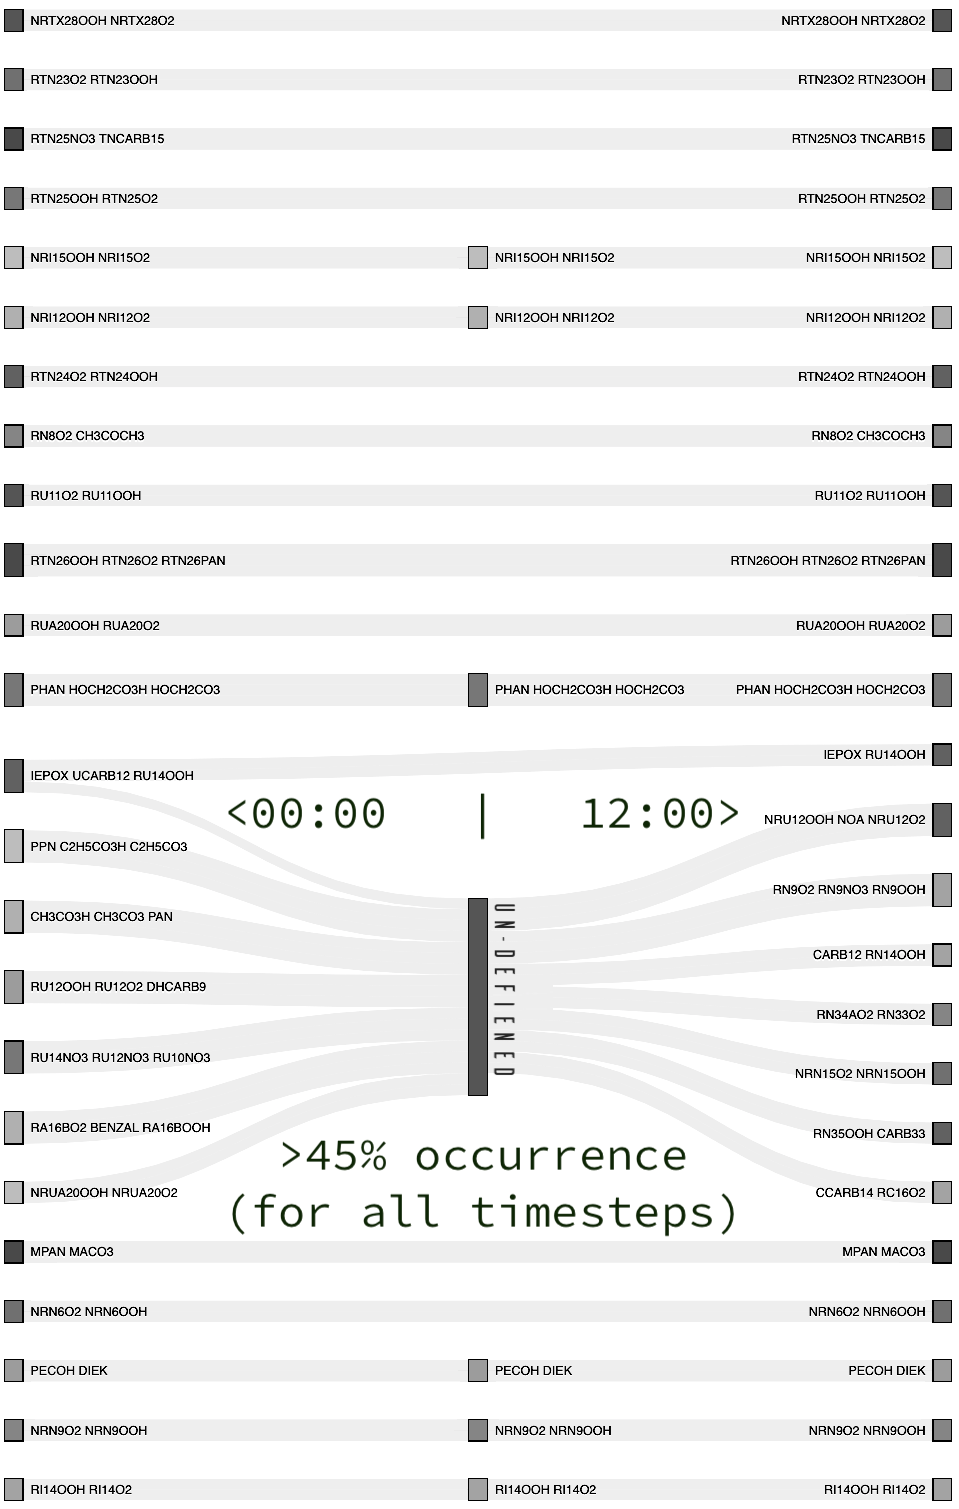
\includegraphics[width=.9\textwidth]{fig/alluvial.png}
\caption{\textbf{An alluvial diagram showing the changes in clusters between noon and midnight.} On the left are all groups that apear in >45\% of the midnight simulation results. On the right are groups which appear >45\% of the midday results. In the middle exist the clusters extracted which appear in >45\% of all runs. Here it is seen that there exist a series of species which may exist in daytime or nighttime chemistry, but do not persist between both. }
\label{fig:alluvial}
\end{figure}



\subsection{Determining cluster suitabiltiy}
Having selected clusters that appear for most graphs in the network, it is now important to assess the suitability of each node for being lumped together. Using a normalised similarity matrix, we extract the values for each of the lumbed groups, \autoref{tab:lumppair}. Here the best values are providec by the PECOH and DIEK species, \autoref{fig:lumppair}a. These both have linear decaying concentrations within the same order of magnitude. This is probably due to PECOH being the only precursor to DIEK, where DIEK accounts for 0.436\% of its total products. This makes them a suitable candidate for lumping. 
\ce{HOCH2CO3H} and \ce{HOCH2CO3} make the worst possible lumping combinations. This is because the radical \ce{HOCH2CO3} is able to react with many of the inorganics, whilst \ce{HOCH2CO3H} can only dissociate into formaldehyde or react with OH to reproduce HOCH2CO3. Although these species both have differing profiles, of several orders of magnitude difference, their cyclic nature \ce{HOCH2CO3H <=>[OH][HO2] HOCH2CO3} most likely proved to trap the `flow' of the network, producing the cluster. Additionally there are also several clusters consisting of \ce{(N)RIxxOOH} and \ce{(N)RIxxO2} species. These are genearally species formed from iso-alkanes, and both produce acetaldehyde (\ce{CH3CHO}) as a product. Here the peroxy radical (\ce{R-O2}) reacts with several inorganic species, producing a varying diurnal. Regardless of this the cosine similarity is still relatively small. This may be attributed to the `flat' periods of slow decay that is experienced at nighttime (due to the reduction of available \ce{HO2} and \ce{NO}) which follow the loss trend of the peroxide (\ce{R-OOH}) species. Since hydrogen addition and subtraction are both fast reactions forming species with the same oxidation potential (or CRI number), it makes sense that the clustering algorithm often identifies peroxides and their peroxy radical equivalent as a group. \\


\begin{table}[H]
\centering
\begin{tabular}{l|cc}
\textbf{Sepecies Pair} & \textbf{Euclidean} & \textbf{Cosine}\\
\hline\hline
NRI15OOH NRI15O2 & 0.4624 & 0.2885 \\
\hline
NRI12OOH NRI12O2 & 0.4617 & 0.2986 \\
\hline
PHAN  HOCH2CO3 & 0.5103 & 0.9998 \\
HOCH2CO3H HOCH2CO3 & 0.8350 & 0.9892 \\
\hline
RI14OOH RI14O2 & 0.4922 & 0.2275 \\
\hline
NRN9O2 NRN9OOH & 0.4620 & 0.2818 \\
\hline
PECOH DIEK & 0.0172 & 0.0011 \\
\end{tabular}
\caption{A table of the \textbf{normalised} similarity values for the lumped species. Numbers closest to 1 show the worst possible paring in the mechanism, and numbers approaching 0 show the best. }
\label{tab:lumppair}
\end{table}


\begin{figure}[H]
\begin{subfigure}[t]{.5\textwidth}
  \centering
  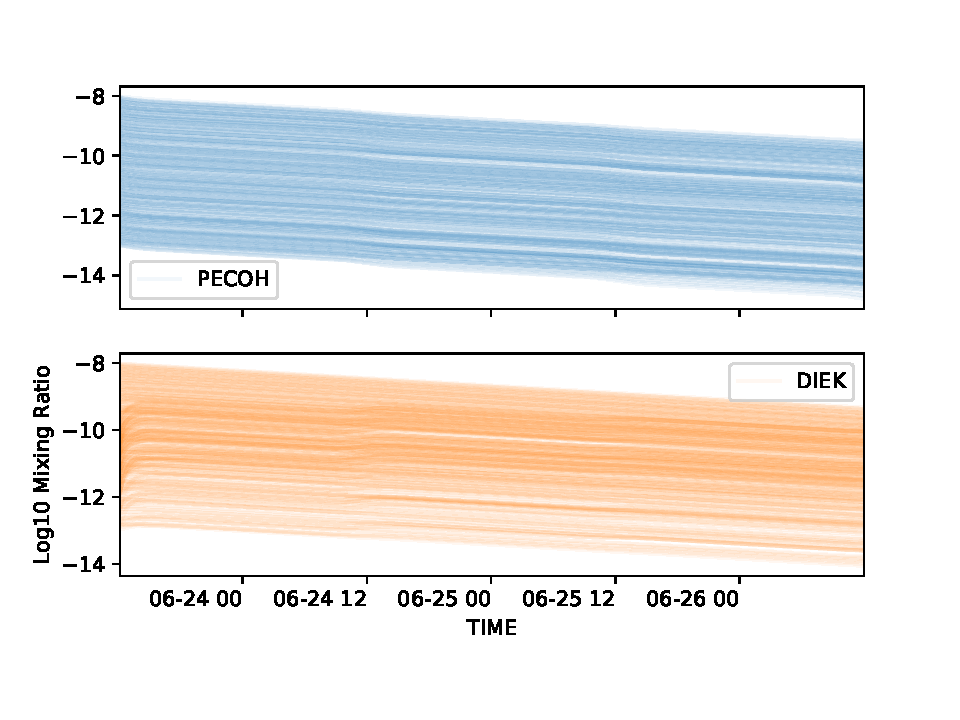
\includegraphics[width=\textwidth]{ensemble/PECOH-DIEK.pdf}
\end{subfigure}%
\begin{subfigure}[t]{.5\textwidth}
  \centering
  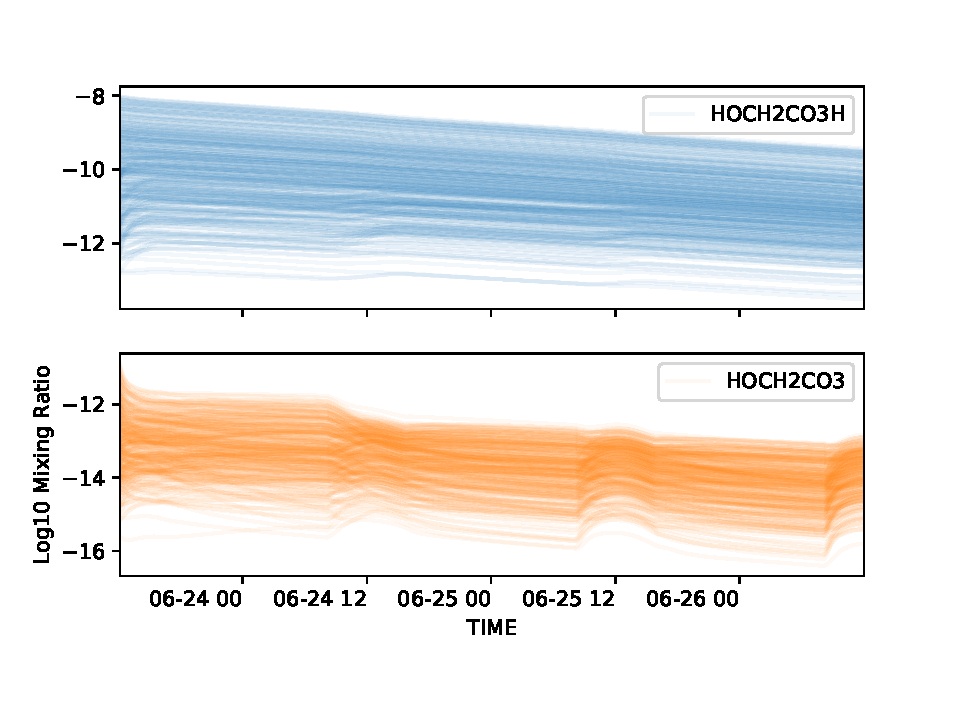
\includegraphics[width=\textwidth]{ensemble/HOCH2CO3H-HOCH2CO3.pdf}
\end{subfigure}%\\

\begin{subfigure}[t]{.5\textwidth}
  \centering
  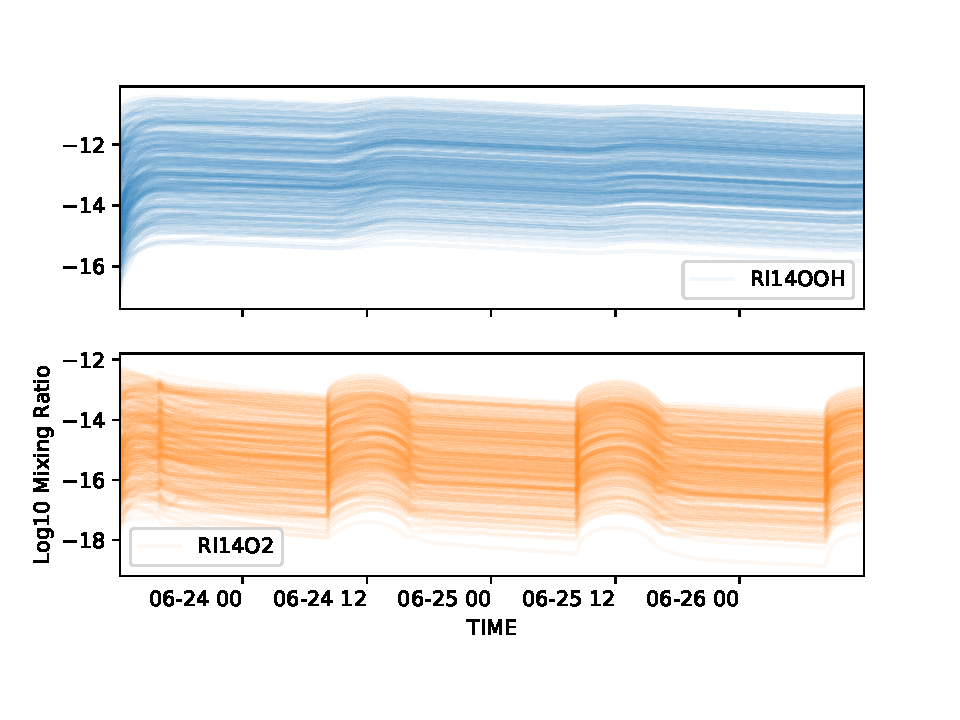
\includegraphics[width=\textwidth]{ensemble/RI14OOH-RI14O2.pdf}
\end{subfigure}%
\begin{subfigure}[t]{.5\textwidth}
  \centering
  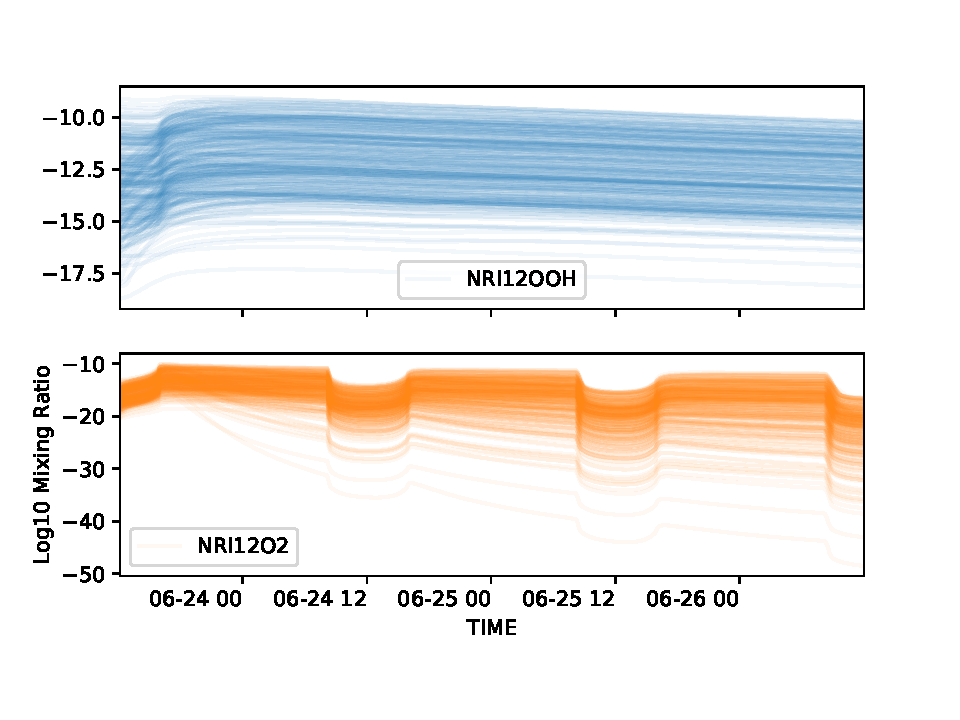
\includegraphics[width=\textwidth]{ensemble/NRI12OOH-NRI12O2.pdf}
\end{subfigure}%\\
\caption{\textbf{Comparing the best (a-b) and worst (c-d) species combinations using the combigned similarity metrics.} }
\label{fig:lumppair}
\end{figure}





% 
% 
% df.index = pd.MultiIndex.from_tuples(... 
% 
% df.euclid = df.euclid/df.euclid.max()
% df.cosine = df.cosine/df.cosine.max()
% 
% 
% 
% g = 'NRI15OOH NRI15O2,,NRI12OOH NRI12O2,,PHAN HOCH2CO3H,PHAN  HOCH2CO3,HOCH2CO3H HOCH2CO3,,RI14OOH RI14O2,,NRN9O2 NRN9OOH,,PECOH DIEK'.split(',')
% 
% 
% s =''
% for i in g:
%     try:
%         e = df.loc[tuple(sorted(i.split()))]
%         s+= '%s & %.4f & %.4f //\n'%(i,e.euclid,e.cosine)
%     except:
%         s+= ' & & //\n'
% 
% 
% print(s)
% 
% 
% g = 'NRI15OOH NRI15O2,NRI12OOH NRI12O2,PHAN HOCH2CO3H HOCH2CO3,RI14OOH RI14O2,NRN9O2 NRN9OOH,PECOH DIEK'.split(',')
% 
% 
% def get(x):
%     import zhdf
%     print (x)
%     return zhdf.new('lhs_general.h5',groupid = x,selection='spec',prodloss=False).spec.compute()
% 
% import multiprocessing as mp
% 
% gps = mp.Pool(50).map(get,range(0,300))
% 
% 
% 
% 
% g = 'RN27OOH RN37OOH,UDCARB20 UDCARB17,UDCARB14 UDCARB17,NRN9O2 NRN9OOH,PECOH DIEK'.split(',')
% 
% g = 'C2H5CO3 CH3NO3,CH3CO3 CH3NO3,MACO3 CH3NO3'.split(',')
% 
% 
% 
% g=['RTX24O2  RTX22O2']
% 
% 
% for i in g:
%     i = i.replace('-',' ').split()
%     print(i)
% 
%     plt.clf()
%     ax = 0
%     del ax
% 
%     for a in gps:
%         alpha = 0.06
%         d = np.log10(a[i])
%         try:
%             ax = d.plot(ax = ax,alpha = alpha,subplots=True,legend=False)
%         except:
%             ax=d.plot(alpha = alpha,subplots=True)
% 
%     plt.ylabel('Log10 Mixing Ratio')
%     plt.savefig('-'.join(i)+'.pdf')







\section{Conculsions}
Graph representation of a chemical network can be used to apply graph clustering techniques. Although there are a range of methods available, the infomap method proves well suited for the use on chemical mechanism. Applying this to the CRI v2.2 mechanism we were able to sucessfully partition the chemistry into branches representing the reactions between differenct chemical structures. This was seen by exploring the hierachical structure of the InfoMap output in the form of a tree. 

Additionally natural language similarity metrics can also apply to compare the temporal changes between species lifetime. Here the Euclidean distance can compare the magnitude difference between species pairs, whilst the cosine distance looks at the angle between them. Combigned these can give us indications if the lumping of two species can prove problematic. 

Finally 300 randomly initiates simulations were compared using  graph clustering. Here persistent groupings were extracted and their suitability compared using the similarity metrics and their lifetimes across the entirety of the simulation. 

Further work would involve the comparison of a mechanism lumped by this method to the unlumped version. The CRI v2.0 mechanism has a series of 5 further lumpings by * and can provide a useful comparison on how beneficial this method of mechanism reductiction fares agains more traditional methods. 
